% Chapter 4

\chapter{Problème 2D et percussion des floes de glace} % 5th chapter title

\label{Chapter4} % For referencing the chapter elsewhere, use \ref{Chapter5} 

%1----------------------------------------------------------------------------------------







\section{Présentation des travaux antérieurs}










% \subsection{Fracture liée un déplacement quasi-statique}

% \subsection{Trajectoire d'un floe percuté}










%2----------------------------------------------------------------------------------------

\section{Dévelopement d'un modèle de percussion}










% \subsection{Déplacement d'un floe isolé}

% Étudions le comportement d'un floe de glace 2D modélisé par un réseau de ressorts (3 ressort, 3 dispositif viseux, et 3 noeuds) (voir \cref{fig:deplacement2d}).
% \begin{figure}[!h]
%     \centering
%     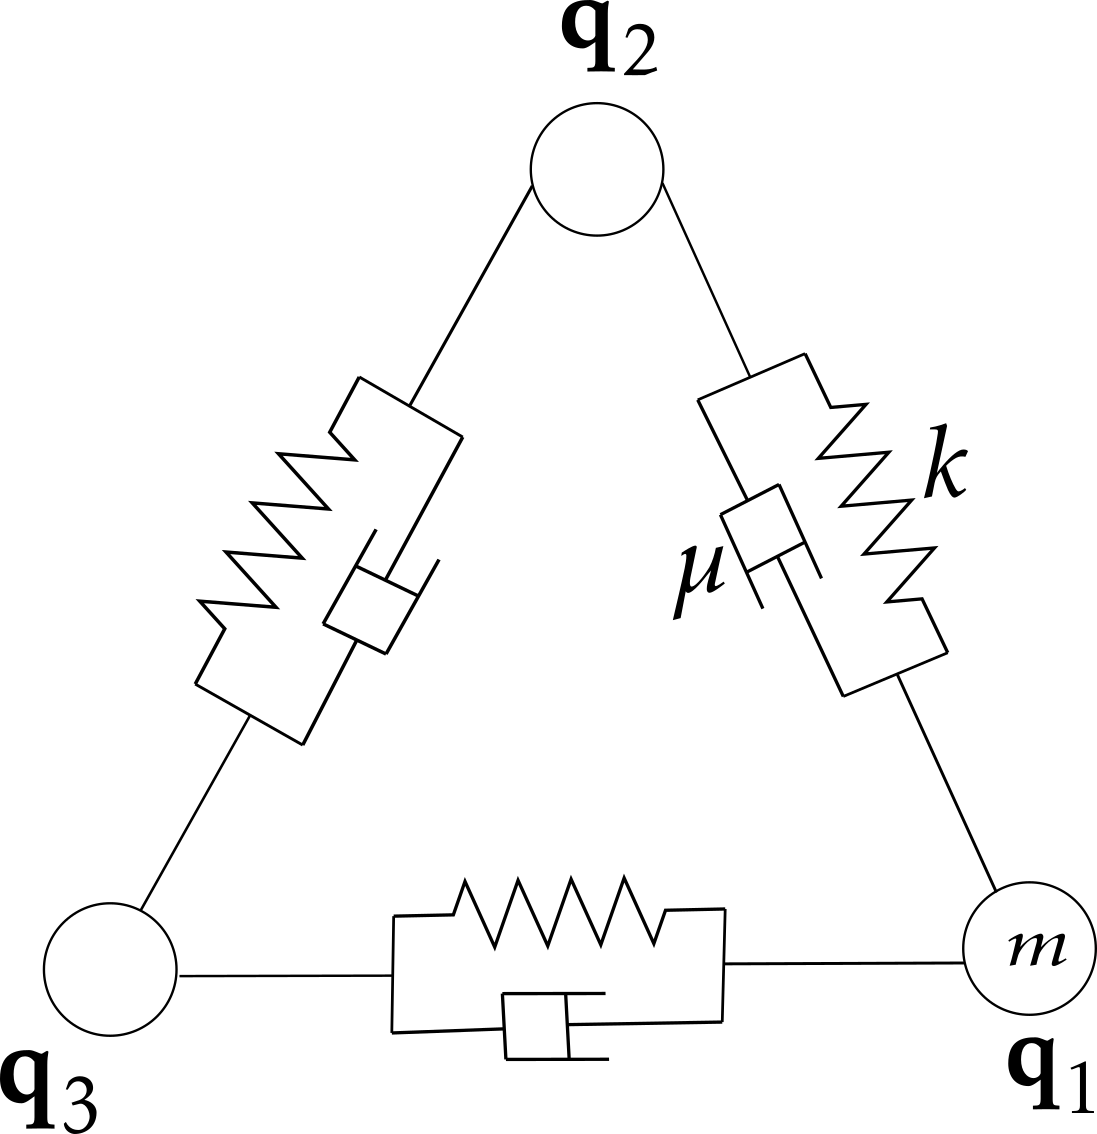
\includegraphics[width=0.3\textwidth]{Deplacement2D-1.png}
%     \caption{Floe de glace 2D modélisé par un réseau de ressorts. Le floe est isolé de toutes forces extérieurs. Tous les neouds du réseau ont la même masse $m$, tous les ressorts on la même raideur $k$, et tous les dispositifs visquens ont le même coefficient $\mu$.}
%     \label{fig:deplacement2d}
% \end{figure}


% \noindent Comme nous l'avons présenté aux \cref{eq:F0,eq:e}, le système de la \cref{fig:deplacement2d} est régit par l' équation:
% \begin{align} \label{eq:eprime2}
%     \forall i \in \mathbb{Z}/3\mathbb{Z}, \quad m \ddot{\bvec{q}}_i = \sum_{j=i+1}^{i+2}C_{ij} \left[  k \left( \Vert \bvec{q}_j - \bvec{q}_i \Vert - L_{ij} \right) \bvec{u}_{ij} - \mu \left\langle \bvec{\dot{q}}_j - \bvec{\dot{q}}_i, \, \bvec{u}_{ij}  \right\rangle  \bvec{u}_{ij}  \right]  , 
% \end{align}
% où $L_{ij}$ représente la longeur au repos du ressort entre les noeuds $i$ et $j$, et $C_{ij}$ indique si les noeuds $i$ et $j$ sont connectés ou non (pour ce modèle 2D simple, $C_{ij} = 1 \, \forall 0 \leq i,j \leq 2$). Le vecteur unitaire $\bvec{u}_{ij}$ vaut:
% $$
% \bvec{u}_{ij} = \frac{\bvec{q}_j - \bvec{q}_i}{\Vert \bvec{q}_j - \bvec{q}_i \Vert}.
% $$


% \paragraph{Simulation par un schéma d'Euler explicite.}

% On discrétise par un schéma de différence finies avec $N+1$ pas de temps, et pour une temps de simulations $T$:
% $$
% \forall i \in \mathbb{Z}/3\mathbb{Z}, \, \forall n \in [\![ 0,N ]\!], \quad  t^n = n\Delta t = n\frac{T}{N}, \quad \bvec{q}_i(t^n) \approx \bvec{q}_i^n.
% $$
% L'\cref{eq:eprime2} devient:
% $$
% m\frac{\bvec{q}_{i}^{n+1}-2\bvec{q}_{i}^{n}+\bvec{q}_{i}^{n-1}}{\Delta t^2} = \sum_{j=i+1}^{i+2}C_{ij}\left[ k \left( \Vert \bvec{q}_j^n - \bvec{q}_i^n \Vert - L_{ij} \right) \bvec{u}_{ij} - \mu \left\langle \frac{\bvec{q}_{j}^{n}-\bvec{q}_{j}^{n-1}}{\Delta t} - \frac{\bvec{q}_{i}^{n}-\bvec{q}_{i}^{n-1}}{\Delta t}, \, \bvec{u}_{ij} \right\rangle  \bvec{u}_{ij}  \right],
% $$
% soit encore:
% \begin{align} \label{eq:systeme2D}
%     \bvec{q}_{i}^{n+1} = 2\bvec{q}_{i}^{n}-\bvec{q}_{i}^{n-1} + \frac{\Delta t^2}{m} \sum_{j=i+1}^{i+2}C_{ij}\left[ k \left( \Vert \bvec{q}_j^n - \bvec{q}_i^n \Vert - L_{ij} \right) \bvec{u}_{ij} - \frac{\mu}{\Delta t} \left\langle \bvec{q}_{j}^{n}-\bvec{q}_{j}^{n-1} - \bvec{q}_{i}^{n}+\bvec{q}_{i}^{n-1}, \, \bvec{u}_{ij} \right\rangle  \bvec{u}_{ij}  \right].
% \end{align}
% La simulation de ce modèle par un schéma d'Euler explicite à pas constant sur un intervalle de temps faible ($T = 4$) est présentée à la \cref{fig:PlotDeplacement2D1Conv}, ainsi que les positions des 2 noeuds au début et à la fin de la simulation. La simulation à la \cref{fig:PlotDeplacement2D1NonConv} permet d'observer le problème avec ce schéma ($T = 10$).


% \begin{figure}[!h]
%     \begin{subfigure}[b]{0.7\textwidth}
%         \centering
%         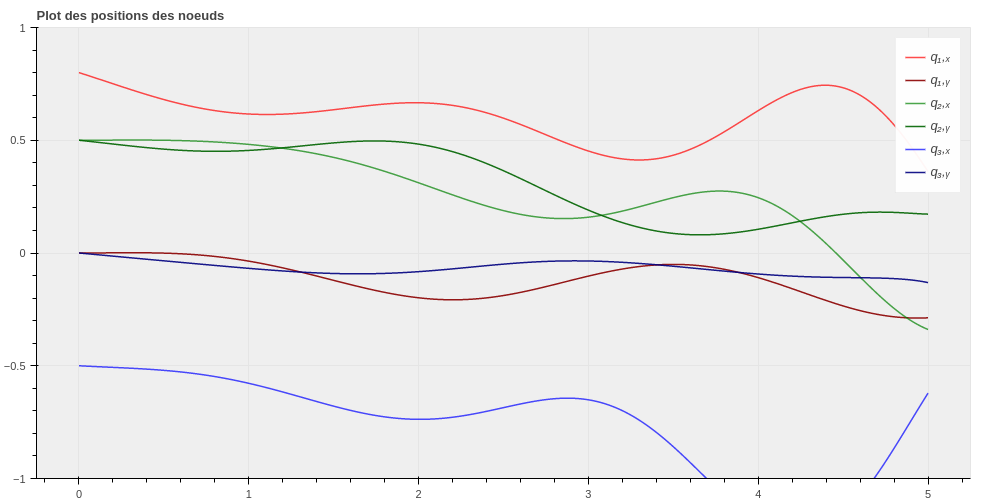
\includegraphics[width=\textwidth]{PlotDeplacement2D-1-Conv.png}
%         \caption{Simulation des positions des noeuds.}
%         \label{fig:dep}
%     \end{subfigure}
% %     \hfill
%     \begin{subfigure}[b]{0.7\textwidth}
%         \centering
%         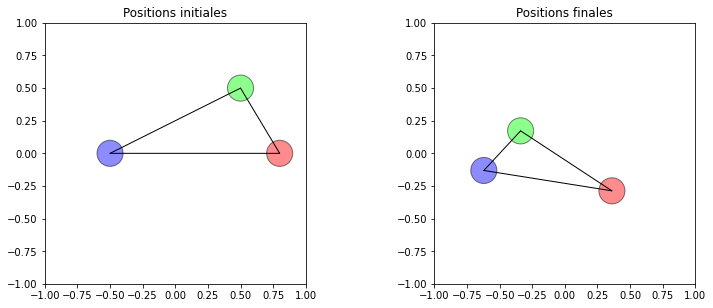
\includegraphics[width=\textwidth]{PositionInitFinales.png}
%         \caption{Illustration des positions initiales et finales des neouds.}
%         \label{fig:pos}
%     \end{subfigure}
%     \caption{Simulation du système \ref{eq:systeme2D} par un schéma d'Euler explicite avec $T = 4$. La couleurs rouge repésente le noeud $\bvec{q}_1$, le vert le noeud $\bvec{q}_2$, le blue le $\bvec{q}_3$. Les paramètres utilisés ici sont les suivants: $m=6.2$, $k=23.3$, $\mu=3$; à l'instant initiale, les trois noeuds perturbés avec des vitesses d'intensité respectives $v_1=0.3$, $v_2=0.1$, et $v_3=0.1$. Par rapport à l'axe des abcisses, ces vitesses ont sont orintées respectivement de $\theta_1=180^\circ$, $\theta_2=270^\circ$, et $\theta_3=240^\circ$ (voir \texttt{code/simu2D/Deplacement2D-1.ipynb}).}
%     \label{fig:PlotDeplacement2D1Conv}
% \end{figure}


% \begin{figure}[!h]
%     \centering
%     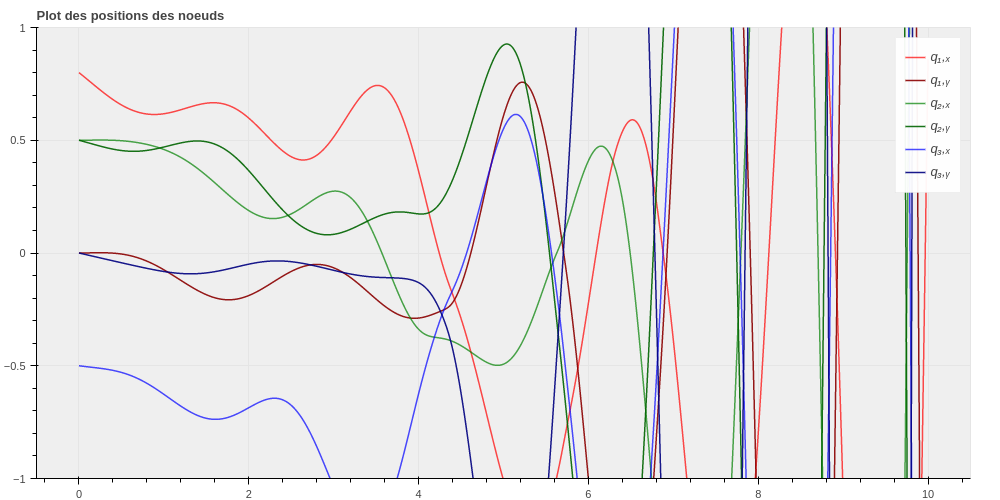
\includegraphics[width=0.7\textwidth]{PlotDeplacement2D-1-NonConv.png}
%     \caption{Simulation du système \ref{eq:systeme2D} par un schéma d'Euler explicite avec $T = 10$. Cette figure utilise les même paramtètres que la \cref{fig:PlotDeplacement2D1Conv}. On observe ici une divergence totale du système.}
%     \label{fig:PlotDeplacement2D1NonConv}
% \end{figure}

% Les \cref{fig:PlotDeplacement2D1Conv,fig:PlotDeplacement2D1NonConv} permettent de constater que le schéma d'Euler explicite (peu importe son pas de temps), n'est pas adapté à ce problème. Nous étudierons donc d'autres alternatives. 

 
% \paragraph{Simulation à l'aide des fonction de la librarie Scipy.} À travers ses fonction telle que \texttt{odeint} et $\verb|solve_ivp|$, \texttt{Scipy} offre une solution robuste et élégante pour simuler les systèmes d'ODE de la forme $Y' = AY$.


 




% \subsection{Modélisation du contact entre deux floes}

% Les floes de glace $\Omega_k$ et $\Omega_l$ sont modélisés par des systèmes masse-ressort (à grande raideur). Pour l'instant, nous considérons une moélisation simplifiée qui assimile un floe à un système de (trois) masses reliés par des ressorts (de constante de raideur $k$), et par des dispositifs visqueux de constante $\mu$.
% Nous désignerons par $n+1$ le nombre total de noeuds du floe $\Omega_k$, chaque noeud ayant pour masse $m$. De facon similaire, on définit les constantes $k'$, $\mu'$, $n'+1$, $m'+1$ pour le floe $\Omega_l$. Les positions des noeds de $\Omega_k$ seront noté $(q_i)_{0\leq i\leq n}$, tandis que ceux de $\Omega_l$ seront notés $(p_i)_{0 \leq i\leq n'}$ (voir \cref{fig:contactmanuel}). 

% \begin{figure}[!h]
%     \centering
%     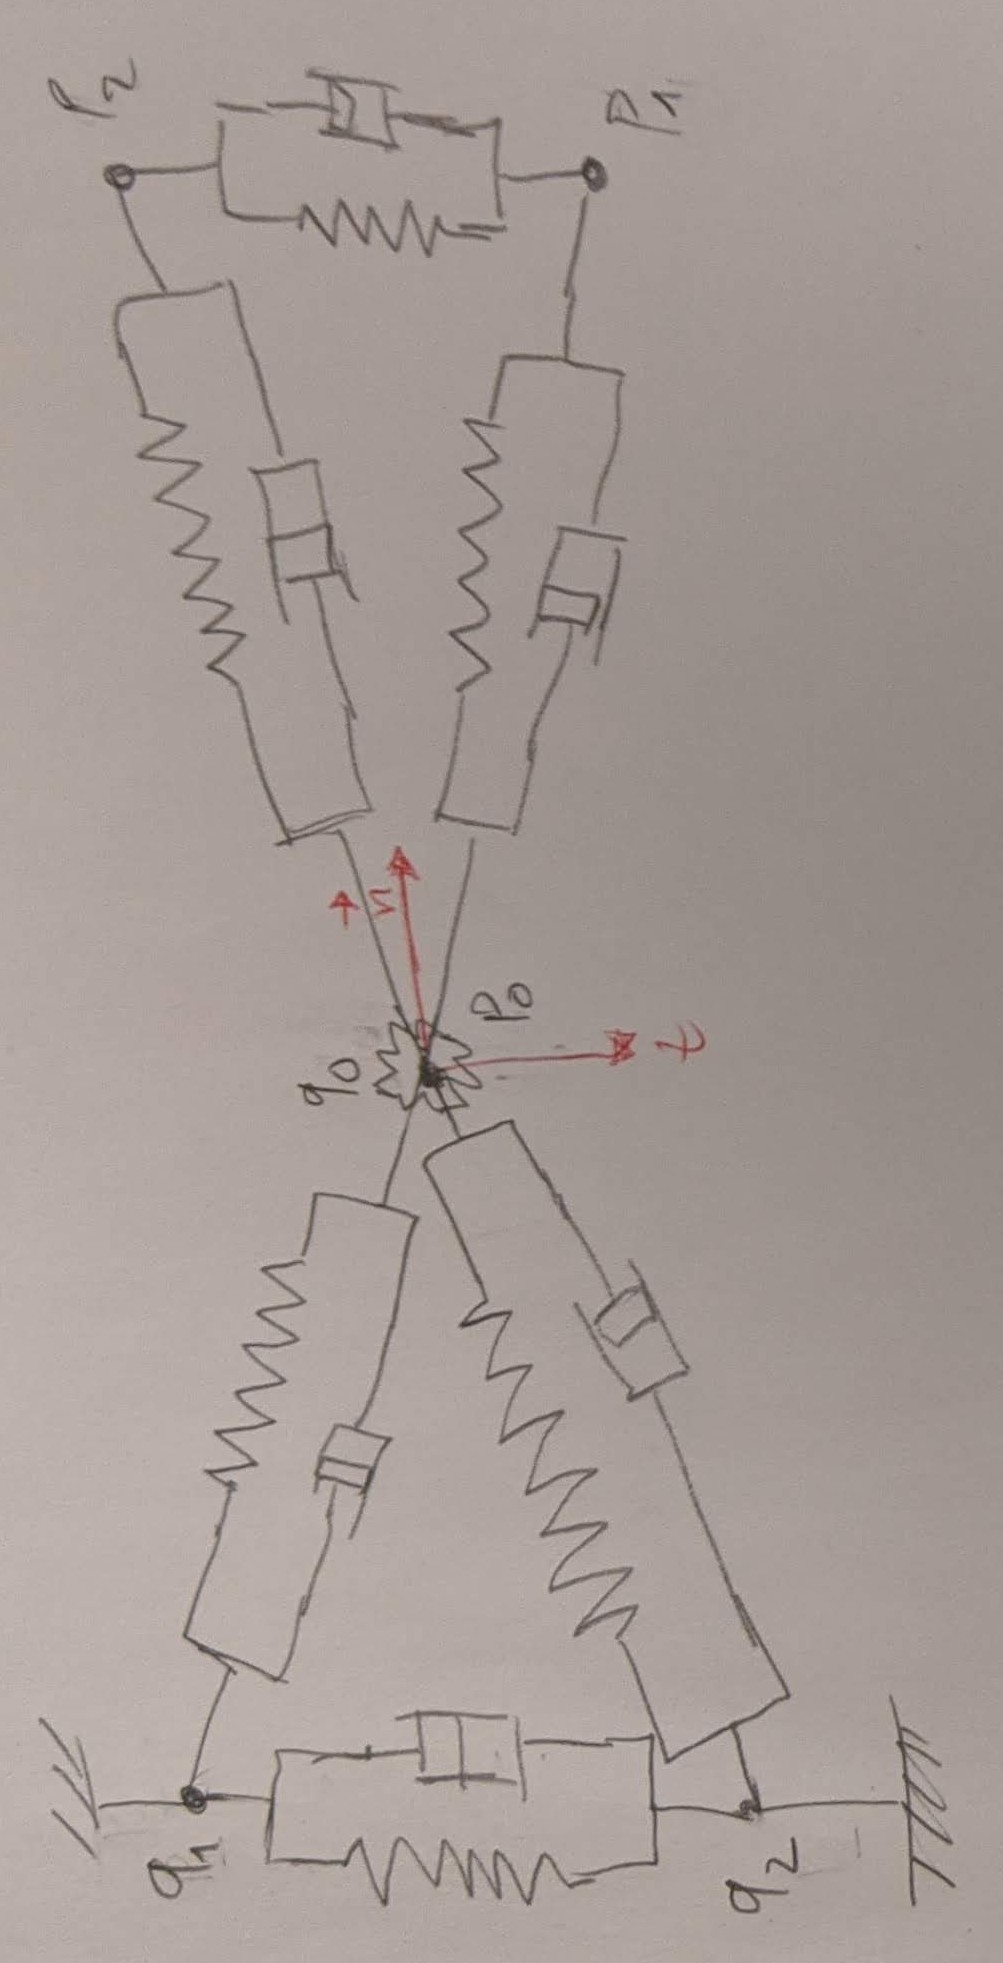
\includegraphics[width=0.3\textwidth, angle=-90]{ContactManuel.jpg}
%     \caption{Contact entre deux floes aux points $p_0 = q_0$.}
%     \label{fig:contactmanuel}
% \end{figure}

% \noindent On définit la matrice de contact $C$...(voir these Dimitri), et $L_{0j}$.. et $u_{0j}$ ..

% \noindent Comme présenté dans les travaux \parencite[p.186]{balasoiu2020halthesis}, le système différentiel qui modélise la percussion s’écrit comme le couplage de deux sous-systèmes. Le premier, dit système intérieur (SI), est à évolution rapide et modélise la propagation des ondes élastiques dans le système masse-ressort. Ici, nous dérivons facilement et réutilisont le SI comme présenté par \citeauthor{balasoiu2020halthesis}. Le second, dit système extérieur (SE), est à évolution lente et modélise la pénétration de l’objet solide dans le système masse-ressorts. Pour dériver le SE sur le floe $\Omega_k$, nous écrivons l'équation de Newton-Euler linéaire\footnote{La rotation du point matériel $q_0$ n'est pas prise en compte ici, d'où l'abscence de l'équation de Newton-Euler angulaire.} au point de contact $q_0$:
% \begin{align}  \label{eq:SE}
% m \ddot{\bvec{q}}_0 = \bvec{F}_0 + \bvec{F}^c_0 \,,
% \end{align}
% où 
% \begin{align}  \label{eq:F0}
%     \bvec{F}_0 = \sum_{j=0}^{n}C_{0j} \left[  \underbrace{k \left( \Vert \bvec{q}_j - \bvec{q}_0 \Vert - L_{0j} \right) \bvec{u}_{0j}}_{\text{Force de rappel}} - \underbrace{\mu \left\langle \bvec{\dot{q}}_j - \bvec{\dot{q}}_0\,, \bvec{u}_{0j}  \right\rangle  \bvec{u}_{0j}}_{\text{Force de dissipation}}  \right] \,,
% \end{align}
% représente la somme des forces de reaction et de disssipation exercées par le ressort et le dispositif visqueux sur le noeud $q_0$ ; et $\bvec{F}^c_0(t)$ la force de contact durant la collison entre les deux particules. En supposnat qu'il existe un repère de contact $\mathcal{R}^c = \{ q_0, \bvec{n}, \bvec{t} \}$ associé au floe $\Omega_k$ (voir \cref{fig:contactmanuel}), on peut écrire, pour $(\lambda, \beta) \in \Rdeux$ :
% \begin{align}  \label{eq:F0c}
%     \bvec{F}_0^c = \lambda \bvec{n} + \beta \bvec{t} \,.
% \end{align}
% Le système intérieur (SE) s'obtient facilement en combinant les équations \cref{eq:SE,eq:F0,eq:F0c}. Le système intérieur (SI) s'obtient lui (pour les autres noeuds du réseau) en y supprimant la force de contact. On obtient au final:
% \begin{align} \tag{$E$} \label{eq:e}
% \begin{dcases}
%     m \ddot{\bvec{q}}_0 = \bvec{F}_0 + \bvec{F}^c_0  \,, &\qquad \text{(SE)} \\
%     m \ddot{\bvec{q}}_i = \bvec{F}_i   \,, \quad \quad \quad \forall 1 \leq i \leq n \,. &\qquad \text{(SI)}
% \end{dcases}
% \end{align}
% En ce qui concerne le floe $\Omega_l$, nous procédons de facons similaire et appliqons la 3ème loi de Newton (action-réaction) pour obtenir le système:
% \begin{align} \tag{$E'$} \label{eq:eprime}
% \begin{dcases}
%     m' \ddot{\bvec{p}}_0 = \bvec{F}^{'}_0 - \bvec{F}^c_0  \,, &\qquad \text{(SE)} \\
%     m' \ddot{\bvec{p}}_i = \bvec{F}^{'}_i   \,, \quad \quad \quad \forall 1 \leq i \leq n' \,, &\qquad \text{(SI)}
% \end{dcases}
% \end{align}
% où $(\bvec{F}^{'}_i)_{0 \leq i \leq n'}$ sont définis de facon similaire à $\bvec{F}_0$ (voir \cref{eq:F0}):
% \begin{align}
%     \bvec{F}'_i = \sum_{j=i}^{n'}C_{ij} \left[ k' \left( \Vert \bvec{p}_j - \bvec{p}_i \Vert - L'_{ij} \right) \bvec{u'}_{ij} - \mu' \left\langle \bvec{\dot{p}}_j - \bvec{\dot{p}}_i\,, \bvec{u}'_{ij}  \right\rangle  \bvec{u}'_{ij}  \right] \,.
% \end{align}

% \noindent Ensuite, on additionne membre à membre les équations des systèmes extérieurs (SE) de \cref{eq:e,eq:eprime} pour éliminer la force de contact. On obtient:
% \begin{align}
% m \ddot{\bvec{q}}_0 + m' \ddot{\bvec{p}}_0 = \bvec{F}_0 + \bvec{F}^{'}_0 \,.
% \end{align}
% Remarquons que les positions relatives des noeuds $\bvec{q}_0$ et $\bvec{p}_0$ restent inchangées durant la collision. A l'instant initial, on note donc $\Delta_0 = \bvec{q}_0(0) - \bvec{p}_0(0)$, et $\bvec{\dot q}_0(0) = \bvec{\dot p}_0(0)$ ; idéalement, nous voudrions que:
% \begin{align}
% \forall t \in \mathbb{R}^+ \,, \quad \bvec{q}_0(t) - \bvec{p}_0(t) = \Delta_0\,.
% \end{align}
% Pour satifaire cette condition, nous exhibons $n+n'+2$ équations nécessaire pour que notre problème de percussion soit bien posé. Elles sont :
% \begin{align} \tag{$\mathcal{P}$} \label{eq:problemeP}
% \begin{dcases}
%     (m+m') \ddot{\bvec{q}}_0  = \bvec{F}_0 + \bvec{F}^{'}_0  \,, &\qquad \text{(SE)} \\
%     \ddot{\bvec{p}}_0 = \ddot{\bvec{q}}_0 \,, &\qquad \text{(SE)} \\
%     m \ddot{\bvec{q}}_i = \bvec{F}_i   \,, \quad \quad \quad \forall 1 \leq i \leq n \,. &\qquad \text{(SI)} \\
%     m' \ddot{\bvec{p}}_i = \bvec{F}^{'}_i   \,, \quad \quad \quad \forall 1 \leq i \leq n' \,, &\qquad \text{(SI)}
% \end{dcases}
% \end{align}

% Ensuite, il nous faut introduire des conditions portant sur la conservation de l'énergie, et la condition de non-interpénétration de Signorini\dots







%3----------------------------------------------------------------------------------------

\section{Présentation du code de calcul 1D}







%4----------------------------------------------------------------------------------------

\section{Résumé des résultats obtenus}

